\hypertarget{tantargyak}{%
\section{Tantárgyak}\label{tantargyak}}

A Budapest School a ma gyerekeinek kínál olyan oktatást, ami segíti
felkészíteni őket a jövő kihívásaira. Információs társadalmunk
legnagyobb kihívása az adaptációs képességünk fejlesztése, ez az alapja
annak, hogy képesek legyünk eligazodni a folyamatosan változó, komplex
világunkban. A tanulásunk célja, hogy boldog, hasznos és egészséges
tagjai legyünk a társadalomnak. Iskolánkban a tanulás három rétege, a
tudásszerzés, a megtanultakat elmélyítő önálló gondolkodás és az aktív
alkotás egyszerre jelennek meg.

Az iskola a célok eléréséhez a NAT tantárgyi struktúráját használja a
tanulás tartalmi keretezéséhez. A keretezésen azt értjük, hogy a
tantárgyak tartalma határozza meg, hogy mivel kell mindenképp foglalkzni a Budapest
School-iskolákban, mit kell mindenképp megtanulni. Az egyes
foglalkozások ezen tantárgyak tanulási eredményeinek elérését
támogatják.

\hypertarget{valasztott-kerettanterv}{%
\subsection{Választott kerettanterv}\label{valasztott-kerettanterv}}

Az iskola a miniszter által közzétett, \emph{Kerettanterv az általános
iskola 1--4., 5--8. és Kerettanterv a gimnáziumok 9--12. évfolyamára} című
tantárgyi kerettantervek {\autocite{Kerettanterv2020}} és a
\emph{Nemzeti alaptanterv} tananyagtartalmát kínálja a gyerekeknek.
Ezek a tantervek adják a tartalmi szabályozás kereteit. Az iskola arra
törekszik, hogy ezt egy minél inkább önvezérelt, személyre szabott
módon tanulják a gyerekek.

Budapest Schoolban a tantárgy a mindennapokban nem feltétlenül jelenik
meg önálló tanóraként. A tantárgy elvégzésének feltétele, hogy a
gyerekek egyéni portfóliója lefedje a NAT-ban tanulási eredményekként
megadott követelményeket.

\hypertarget{tanulasi-eredmenyek-a-formalis-tanulas-alapegysegei}{%
\subsection{Tanulási eredmények --- a formális tanulás
alapegységei}\label{tanulasi-eredmenyek-a-formalis-tanulas-alapegysegei}}

Az iskola a NAT \emph{tanulási eredményeit} veszi alapul. A tanulási
eredmények (learning outcomes) tudás, képesség, kompetencia, attitűd
kontextusában meghatározott kijelentések arra vonatkozóan, hogy a
tanulónak mit kell tudnia, mit kell értenie, és mire legyen képes,
miután lezárt egy tanulási folyamatot, függetlenül attól, hogy hol,
hogyan, mikor szerezte meg ezeket a kompetenciákat
{\autocite{Cedefop2008}}

Az eredmény elérésé a tanulási-tanítási egységeken, a \emph{modulokon}
keresztül vagy az egyéni, önálló tanulás alapján történik. A tanulás
folyamata történhet az iskolában vagy azon kívül, lehet formális,
nem-formális vagy informális. Az iskola támogatja a tanárokat abban a
céljukban, hogy minél differenciáltabb, gyerekekre szabott módon
tudják segíteni a tantárgyi anyag elsajátítását. Az egyes
tanulási-tanítási egységek, a modulok különféle tanulási eredmények
elérését is támogathatják, ezzel több tantárgy részcéljait is
teljesíthetik.

A tanulási eredmények több funkciót látnak el a BPS modellben.

\begin{itemize}
\item
  A tanulási eredmények a modulok (és így a mindennapokban szervezett
  foglalkozások, órák stb.) építőelemei. Egy-egy modul célját a
  tanulásszervezők az elérendő tanulási eredmények összeválogatásával és
  saját célokkal, érdeklődéssel kiegészítve adják meg, figyelembe véve
  az életkori sajátosságok, az egymásra épülés és az átjárhatóság
  követelményeit.
\item
  Egy gyerek akkor
  léphet a következő évfolyamra
  (\ref{evfolyam}.~fejezet, \pageref{evfolyam}. oldal),
  ha a tantárgyhoz tartozó követelményeket teljesítette.
\item
  A tanulási eredmények alapján
  az osztályzatok (\ref{erdemjegyek-es-osztalyzatok}.~fejezet, \pageref{erdemjegyek-es-osztalyzatok}.~oldal)
  egy átlátható és egyszerű számítás segítségével megállapíthatók.
\end{itemize}

A BPS modell tantárgyankénti bontásban adja meg a továbbhaladáshoz
elengedhetetlen tanulási eredmények halmazát, amik teljesen megfelelnek
a NAT tanulási eredményeinek. Ezek adják a követelményeket, a kereteket.
A NAT (és a közzétett kerettantervek) témakörei ajánlások; ahogy a
jogszabály fogalmaz, \emph{sorrendjük változtatható és koherens
rendszerbe építhető}. Ezt a rendszert alakítják ki a tanárok a
tanulási-tanítási egységek, a modulok során, és a gyerekek az egyéni
tanulás alkalmával.

Két tanár, két osztály vagy két gyerek között a tanmenet tekintetében
akár jelentős eltérések lehetnek addig, amig a NAT tanulási eredményei
teljesülnek. A tanulási eredményen alapuló szabályozás folyamatos
visszacsatolást tud adni a tanulónak és a tanároknak, megmutatva, melyik
tanulási eredményeket kell még elérni a következő szintre való lépéshez.

\hypertarget{tantargyi-oraszamok}{%
\subsection{Tantárgyi óraszámok}\label{tantargyi-oraszamok}}

{
\let\tabularnewline\cr
\vbox{%
  \offinterlineskip
  \halign{%
    #\hfil\strut\ &\vrule\ \hfil#\strut\ &\vrule\ \hfil#\strut\ &\vrule\ \hfil#\strut\ &\vrule\ \hfil#\strut\ &\vrule\ \hfil#\strut\ &\vrule\ \hfil#\strut\ &\vrule\ \hfil#\strut\ &\vrule\ \hfil#\strut\ &\vrule\ \hfil#\strut\ &\vrule\ \hfil#\strut\ &\vrule\ \hfil#\strut\ &\vrule\ \hfil#\strut\ &\vrule#\cr
\bfseries Tantárgy &\bfseries  1 &\bfseries  2 &\bfseries  3 &\bfseries  4 &\bfseries  5 &\bfseries  6 &\bfseries  7 &\bfseries  8 &\bfseries  9 &\bfseries  10 &\bfseries  11 &\bfseries 
12&\tabularnewline
\noalign{\hrule}
% \endhead
Állampolgári & & & & & & & & & & & & &\tabularnewline
\quad ismeretek & & & & & & & & 1 & & & & 1&\tabularnewline
\noalign{\hrule}
Biológia & & & & & & & & & 3 & 2 & &&\tabularnewline
\noalign{\hrule}
Digitális kultúra & & & 1 & 1 & 1 & 1 & 1 & 1 & 2 & 1 & 2
&&\tabularnewline
\noalign{\hrule}
Dráma és színház & & & & & & & 1 & & & & &&\tabularnewline
\noalign{\hrule}
Első idegen nyelv & & & & 2 & 3 & 3 & 3 & 3 & 3 & 3 & 4 &
4&\tabularnewline
\noalign{\hrule}
Ének-zene & 2 & 2 & 2 & 2 & 2 & 1 & 1 & 1 & 1 & 1 & &&\tabularnewline
\noalign{\hrule}
Etika & 1 & 1 & 1 & 1 & 1 & 1 & 2 & 2 & & & &&\tabularnewline
\noalign{\hrule}
Fizika & & & & & & & & & 2 & 3 & &&\tabularnewline
\noalign{\hrule}
Földrajz & & & & & & & & & 2 & 1 & &&\tabularnewline
\noalign{\hrule}
Hon- és népismeret & & & & & & 1 & & & & & &&\tabularnewline
\noalign{\hrule}
Kémia & & & & & & & & & 1 & 2 & &&\tabularnewline
\noalign{\hrule}
Környezetismeret & & & 1 & 1 & & & & & & & &&\tabularnewline
\noalign{\hrule}
Magyar nyelv és & & & & & & & & & & & & &\tabularnewline
\quad irodalom & 7 & 7 & 5 & 5 & 4 & 4 & 3 & 3 & 3 & 4 & 4 &
4&\tabularnewline
\noalign{\hrule}
Második idegen nyelv & & & & & & & & & 3 & 3 & 3 & 3&\tabularnewline
\noalign{\hrule}
Matematika & 4 & 4 & 4 & 4 & 4 & 4 & 3 & 3 & 3 & 3 & 3 &
3&\tabularnewline
\noalign{\hrule}
Mozgóképkultúra és & & & & & & & & & & & & &\tabularnewline
\quad médiaismeret & & & & & & & & & & & & 1&\tabularnewline
\noalign{\hrule}
Technika és tervezés & 1 & 1 & 1 & 1 & 1 & 1 & 1 & & & &
&&\tabularnewline
\noalign{\hrule}
Természettudomány & & & & & 2 & 2 & 4 & 5 & & & 2 &&\tabularnewline
\noalign{\hrule}
Testnevelés és & & & & & & & & & & & & &\tabularnewline
\quad egészségfejlesztés & 5 & 5 & 5 & 5 & 5 & 5 & 5 & 5 & 5 &
5 & 5 & 5&\tabularnewline
\noalign{\hrule}
Történelem & & & & & 2 & 2 & 2 & 2 & 2 & 2 & 3 & 3&\tabularnewline
\noalign{\hrule}
Vizuális kultúra & 2 & 2 & 2 & 1 & 1 & 1 & 1 & 1 & 1 & 1 &
&&\tabularnewline
\noalign{\hrule}
Mentoridő & 1 & 1 & 1 & 1 & 1 & 1 & 1 & 1 & 1 & 1 & 1 & 1&\tabularnewline
\noalign{\hrule}
Kötött célú órakeret & & & & & & & & & & & 4 & 4&\tabularnewline
% & & & & & & & & & & & &\tabularnewline
\noalign{\hrule}
\emph{Összesen} & 23 & 23 & 23 & 24 & 27 & 27 & 28 & 28 & 32 & 32 & 31 &
29&\tabularnewline
\noalign{\hrule}
}
}
}



%% \newcolumntype{L}{>{\begin{minipage}[t]{.2\textwidth}\strut\raggedright\hangindent=1em}l<{\strut\end{minipage}}}
%% \begin{longtable}[]{L*{12}{|r}}
%% \renewcommand{\arraystretch}{1.5}
%% Tantárgy & 1 & 2 & 3 & 4 & 5 & 6 & 7 & 8 & 9 & 10 & 11 &
%% 12\tabularnewline
%% \hline
%% \endhead
%% Állampolgári ismeretek & & & & & & & & 1 & & & & 1\tabularnewline
%% Biológia & & & & & & & & & 3 & 2 & &\tabularnewline
%% Digitális kultúra & & & 1 & 1 & 1 & 1 & 1 & 1 & 2 & 1 & 2
%% &\tabularnewline
%% Dráma és színház & & & & & & & 1 & & & & &\tabularnewline
%% Első idegen nyelv & & & & 2 & 3 & 3 & 3 & 3 & 3 & 3 & 4 &
%% 4\tabularnewline
%% Ének-zene & 2 & 2 & 2 & 2 & 2 & 1 & 1 & 1 & 1 & 1 & &\tabularnewline
%% Etika & 1 & 1 & 1 & 1 & 1 & 1 & 2 & 2 & & & &\tabularnewline
%% Fizika & & & & & & & & & 2 & 3 & &\tabularnewline
%% Földrajz & & & & & & & & & 2 & 1 & &\tabularnewline
%% Hon- és népismeret & & & & & & 1 & & & & & &\tabularnewline
%% Kémia & & & & & & & & & 1 & 2 & &\tabularnewline
%% Környezetismeret & & & 1 & 1 & & & & & & & &\tabularnewline
%% Magyar nyelv és irodalom & 7 & 7 & 5 & 5 & 4 & 4 & 3 & 3 & 3 & 4 & 4 &
%% 4\tabularnewline
%% Második idegen nyelv & & & & & & & & & 3 & 3 & 3 & 3\tabularnewline
%% Matematika & 4 & 4 & 4 & 4 & 4 & 4 & 3 & 3 & 3 & 3 & 3 &
%% 3\tabularnewline
%% Mozgóképkultúra és médiaismeret & & & & & & & & & & & & 1\tabularnewline
%% Technika és tervezés & 1 & 1 & 1 & 1 & 1 & 1 & 1 & & & &
%% &\tabularnewline
%% Természettudomány & & & & & 2 & 2 & 4 & 5 & & & 2 &\tabularnewline
%% Testnevelés és egészségfejlesztés & 5 & 5 & 5 & 5 & 5 & 5 & 5 & 5 & 5 &
%% 5 & 5 & 5\tabularnewline
%% Történelem & & & & & 2 & 2 & 2 & 2 & 2 & 2 & 3 & 3\tabularnewline
%% Vizuális kultúra & 2 & 2 & 2 & 1 & 1 & 1 & 1 & 1 & 1 & 1 &
%% &\tabularnewline
%% Mentoridő & 1 & 1 & 1 & 1 & 1 & 1 & 1 & 1 & 1 & 1 & 1 & 1\tabularnewline
%% Kötött célú órakeret & & & & & & & & & & & 4 & 4\tabularnewline
%% & & & & & & & & & & & &\tabularnewline
%% \emph{Összesen} & 23 & 23 & 23 & 24 & 27 & 27 & 28 & 28 & 32 & 32 & 31 &
%% 29\tabularnewline
%% \bottomrule
%% \end{longtable}

%% \begin{longtable}[]{@{}lrrrrrrrrrrrr@{}}
%% \toprule
%% Tantárgy & 1 & 2 & 3 & 4 & 5 & 6 & 7 & 8 & 9 & 10 & 11 &
%% 12\tabularnewline
%% \midrule
%% \endhead
%% Állampolgári ismeretek & & & & & & & & 1 & & & & 1\tabularnewline
%% Biológia & & & & & & & & & 3 & 2 & &\tabularnewline
%% Digitális kultúra & & & 1 & 1 & 1 & 1 & 1 & 1 & 2 & 1 & 2
%% &\tabularnewline
%% Dráma és színház & & & & & & & 1 & & & & &\tabularnewline
%% Első idegen nyelv & & & & 2 & 3 & 3 & 3 & 3 & 3 & 3 & 4 &
%% 4\tabularnewline
%% Ének-zene & 2 & 2 & 2 & 2 & 2 & 1 & 1 & 1 & 1 & 1 & &\tabularnewline
%% Etika & 1 & 1 & 1 & 1 & 1 & 1 & 2 & 2 & & & &\tabularnewline
%% Fizika & & & & & & & & & 2 & 3 & &\tabularnewline
%% Földrajz & & & & & & & & & 2 & 1 & &\tabularnewline
%% Hon- és népismeret & & & & & & 1 & & & & & &\tabularnewline
%% Kémia & & & & & & & & & 1 & 2 & &\tabularnewline
%% Környezetismeret & & & 1 & 1 & & & & & & & &\tabularnewline
%% Magyar nyelv és irodalom & 7 & 7 & 5 & 5 & 4 & 4 & 3 & 3 & 3 & 4 & 4 &
%% 4\tabularnewline
%% Második idegen nyelv & & & & & & & & & 3 & 3 & 3 & 3\tabularnewline
%% Matematika & 4 & 4 & 4 & 4 & 4 & 4 & 3 & 3 & 3 & 3 & 3 &
%% 3\tabularnewline
%% Mozgóképkultúra és médiaismeret & & & & & & & & & & & & 1\tabularnewline
%% Technika és tervezés & 1 & 1 & 1 & 1 & 1 & 1 & 1 & & & &
%% &\tabularnewline
%% Természettudomány & & & & & 2 & 2 & 4 & 5 & & & 2 &\tabularnewline
%% Testnevelés és egészségfejlesztés & 5 & 5 & 5 & 5 & 5 & 5 & 5 & 5 & 5 &
%% 5 & 5 & 5\tabularnewline
%% Történelem & & & & & 2 & 2 & 2 & 2 & 2 & 2 & 3 & 3\tabularnewline
%% Vizuális kultúra & 2 & 2 & 2 & 1 & 1 & 1 & 1 & 1 & 1 & 1 &
%% &\tabularnewline
%% Mentoridő & 1 & 1 & 1 & 1 & 1 & 1 & 1 & 1 & 1 & 1 & 1 & 1\tabularnewline
%% Kötött célú órakeret & & & & & & & & & & & 4 & 4\tabularnewline
%% & & & & & & & & & & & &\tabularnewline
%% \emph{Összesen} & 23 & 23 & 23 & 24 & 27 & 27 & 28 & 28 & 32 & 32 & 31 &
%% 29\tabularnewline
%% \bottomrule
%% \end{longtable}

\newpage

\begin{itemize}
\tightlist
\item
  \emph{Hon- és népismeret} tantárgy a 6. évfolyamon van.
\item
  A \emph{Biológia}, \emph{Fizika}, \emph{Földrajz} és \emph{Kémia}
  diszciplináris tartalmak az iskola 7. és 8. évfolyamán egy integrált
  \emph{Természettudomány} tantárgy részeként jelennek meg.
\item
  A \emph{Második idegennyelv} tantárgy célja, hogy a gyerekek a 12.
  évfolyam végére elérjék a KER szerinti A2 szintet.
\item
  A 12. évfolyamon az iskola a \emph{Mozgóképkultúra és médiaismeret}
  tantárgyat választja.
\item
  Közösségi nevelés (osztályfőnöki) tantárgy helyett heti egy óra
  \emph{mentoridőt} kap minden gyerek.
\end{itemize}

A BPS modell a NAT tantárgyi követelményeihez és technikum esetén a
Képzési és Kimeneti Követelményekhez a tanulási eredményeken keresztül
kapcsolódik. A modell nem köti meg, hogyan éri a gyerek az eredményt,
csak hogy mit kell elérnie. Ezért a tantárgyi óraszámok szerepe
harmadrendű az iskolában.

A modulok során több tantárgyi tananyagot is érinthetnek a modul
résztvevői. Egy modul így több tantárgyi órát is lefedhet, ráadásul ez
óra\-szám-meg\-takarítással is jár. 5 óra angolul tartott drámafoglalkozás
egyszerre számíthat 5 óra \emph{magyar nyelv és irodalom} és 5 óra
\emph{idegennyelv} órának.

A modulok tantárgyi óraszámát a teljes modul hosszára kell számítani, nem
pedig hetente. Egy összevont természettudományi modul, ami érinti a kémiát
és a fizikát is, nem kell, hogy minden héten járjon kémia tanulási
eredménnyel. Több tantárgyat lefedő modul esetén a tantárgyi óraszámokat
úgy kell számolni, hogy először meg kell állapítani, hogy átlagban az
idő hány százalékában foglalkozik a modul egy-egy tantárgy anyagával,
majd a modul teljes hosszából becsülhető a tantárgyi óraszám. Például
egy \emph{tudományos kísérletezés} modul során az idő 30\%-ában
foglalkozunk kémiával, 40\%-ában fizikával, és 30\%-ában
szociálpszichológiával. A modul egy trimeszteren keresztül tart,
kéthetente 4 órában. Ebből számolható a modul teljes hossza, ami itt
12/2~$\times$~4~=~24 óra. Ez hetente 24~$\times$~0,3~=~7,2 óra kémiának és 7,2 óra
fizikának felel meg.

Az önálló tanulás tantárgyi óraszámait nem lehet ilyen egyszerűen
tantárgyi óraszámokra leképezni, mert ehhez minden gyerek minden
pillanatában rögzíteni kéne, hogy akkor éppen melyik tantárgy tananyagával
foglalkozik.

A tanulás tantárgyak szerinti eloszlását az iskola folyamatosan követi,
és gyerekenként, illetve évfolyamonként képes kimutatást készíteni egy
adott időszakban a tantárgyi óraszámok teljesüléséről.

\hypertarget{tantargyakMentorido}{%
\paragraph{Mentoridő}\label{tantargyakMentorido}}

Minden gyerek egy órát hetente a mentorával tölt, amikor a mentor a
gyerek számára egyéni, minőségi figyelmet ad. A mentor ilyenkor a
gyereket segíti a saját céljainak megfogalmazásában, és abban, hogy legyen
lehetősége reflektálni a saját fejlődésére. Ez az óra a gyerekek és a
mentorok számára kötelező foglalkozás.

\hypertarget{a-valasztott-kerettanterv-altal-meghatarozott-oraszam-feletti-kotelezo-tanorai-foglalkozasok}{%
\subsubsection{A választott kerettanterv által meghatározott óraszám
feletti kötelező tanórai
foglalkozások}\label{a-valasztott-kerettanterv-altal-meghatarozott-oraszam-feletti-kotelezo-tanorai-foglalkozasok}}

A BPS modell nem határoz meg kötelező tanórai foglalkozásokat. A modell
azt szeretné, ha a gyerekek minél inkább azt tanulnák, amire nekik
szükségük van, vagy amit szeretnének. Az iskola biztosítja, hogy minden
gyerek megismerkedjen az
elsősegéllyel (\ref{elsosegely-nyujtasi-alapismeretek}.~fejezet, \pageref{elsosegely-nyujtasi-alapismeretek}.~oldal),
a körülötte éle
nemzetiségekkel (\ref{nemzetisegek-megismerese}.~fejezet, \pageref{nemzetisegek-megismerese}.~oldal)
és legyen lehetősége
mindennapos testmozgásra (\ref{mindennapos-testmozgas}.~fejezet, \pageref{mindennapos-testmozgas}.~oldal).

\hypertarget{a-kerettantervben-meghatarozottakon-felul-a-nem-kotelezo-tanorai-foglalkozasok}{%
\subsubsection{A kerettantervben meghatározottakon felüli nem kötelező
tanórai
foglalkozások}\label{a-kerettantervben-meghatarozottakon-felul-a-nem-kotelezo-tanorai-foglalkozasok}}

A kerettantervben meghatározottakon felül az iskola nem határoz meg
előre nem kötelező tanórai foglalkozásokat, ezért azok megtanítandó és
elsajátítandó tananyaga, az ehhez szükséges kötelező, kötelezően
választandó vagy szabadon választható tanórai foglalkozások megnevezése,
óraszáma nincs rögzítve. A tanulásszervező tanárok új foglalkozásokat
hirdethetnek.

\hypertarget{a-tantargyak-szerepe-a-mindennapokban}{%
\subsection{A tantárgyak szerepe a
mindennapokban}\label{a-tantargyak-szerepe-a-mindennapokban}}

A Budapest School iskoláiban a tantárgyak ugyanúgy kapnak szerepet, mint
a NAT által definiált kulcskompetenciák, fejlesztési területek: a tanár
nem mondja azt a gyerekeknek, hogy „most kezdeményezőképességet és
vállalkozói kompetenciát fejlesztünk''; a fejlesztés a különböző feladatok
elvégzésének eredménye. A Budapest School-iskolákban a komplex tevékenységek vannak előtérben. A tantárgyak a
tanulás tartalmi elemeinek forrásai és keretei: a tanulandó dolgok
halmazaként működnek. Az, hogy milyen csoportosításban történik a
tanulás, az a tanárokra és (felsőtől) a gyerekekre van bízva.

A tantárgyak ezért elsősorban a tanulási-tanítási egységek
kialakításakor, a modulok kiírásakor és azok kimeneti értékelésekor
jelennek meg, a mindennapok struktúráját, a napi- és hetirendet azonban
a modulok adják. Egyes modulok több tantárgy fejlesztési céljainak is
eleget tehetnek, több tantárgy tanulási eredményének elérését is célul
tűzhetik ki, összhangban a NAT-tal. A tantárgyaknak ezzel együtt fontos
célja, hogy segítsék a tanulás tartalmi egyensúlyának fennmaradását.

Minden tanulási-tanítási egység, azaz modul lezártakor külön értékelni
kell a tantárgyankénti tudáselsajátítást. Tulajdonképpen nem történik
más, mint például az, hogy egy összevont természettudományi foglalkozássorozat végén
értékeljük, hogy mennyit fejlődött a gyerek tudása külön matematikából,
biológiából, kémiából és fizikából.

\hypertarget{modulok-es-tanulasi-eredmenyek}{%
\subsection{Modulok és tanulási
eredmények}\label{modulok-es-tanulasi-eredmenyek}}

A gyerekek egyik feladata az iskolában, hogy tanulási eredményeket
érjenek el. Ezt megtehetik a modulok elvégzésével vagy más tanulási
helyzetekben. A tanulási eredményeket a portfólióban rögzítik. A mentor
feladata, hogy folyamatosan kövesse, hogy megfelelő haladás történik-e a
portfólióban a tanulási eredmények és a saját célok tekintetében. A gyerek
csak akkor léphet a következő évfolyamra, ha az
évfolyam teljesítéséhez szükséges tanulási eredményeket elérte (\ref{evfolyam}.~fejezet, \pageref{evfolyam}.~oldal).

A modul a gyerekek haladásához releváns tanulási
eredményekkel kecsegtet, a gyerekeknek meghatározott saját céljai
vannak, és a modul
kimenete a portfólióban rögzíthető, legyen az egy alkotás, az
elért fizikai vagy szellemi eredmény dokumentációja vagy egy értékelő
visszajelzés. A modulok tehát tartalmaznak tanulási eredményeket, az
önálló gondolkodás, szabad alkotás lehetőségét, és teret engednek az
alkotásra, létrehozásra.

\hypertarget{a-modulok-kulonfele-tanulasi-eredmenyek-elereset-teszik-elerhetove}{%
\paragraph{A modulok különféle tanulási eredmények elérését teszik
elérhetővé}\label{a-modulok-kulonfele-tanulasi-eredmenyek-elereset-teszik-elerhetove}}\hfil\break
A modulok tervezésekor és összeállításakor a tanulásszervezők a
szaktanárokkal közösen határozzák meg a modul céljait, de azok
meghirdetéséért mindig a tanulásszervezők felelnek. A célok között fel
kell sorolni, hogy milyen tanulási eredmények elérését várhatják el a
gyerekek a modulon való részvételtől.

Például a 6--8 éves gyerekek számára megtervezett „\emph{3d nyomtató
használata}'' modul során azon kívül, hogy megismerik a 3d nyomtatás
folyamatát, a modul célja, hogy a gyerekek számára elérhetővé tegye a
\emph{``Megfigyeli a kocka mint speciális téglatest és a négyzet mint
speciális téglalap tulajdonságait''} (Matematika tantárgy, 1--4.
évfolyam) tanulási eredményt is.

Arra is van lehetőség, hogy egy modulban több tantárgyhoz tartozó
tanulási eredményt is kiválasszunk, ezzel biztosítva az interdiszciplinaritást, valamint a
Budapest School
kiemelt fejlesztési területeihez (\ref{kiemelt-fejlesztesi-teruletek}.~fejezet, \pageref{kiemelt-fejlesztesi-teruletek}.~oldal)
való integrált kapcsolódást.

A tanulási eredmények időbeli egymásra épülést feltételeznek,
melyben azonban van lehetőség előre- és hátrafelé is lépni. Előre,
amenynyiben a modul meghirdetésekor az arra jelentkező gyerekcsoportnál
a megfelelő előkészítés megtörtént, hátra, amennyiben ezt
ismétlés\slash felzárkóztatás jelleggel szükségesnek ítéli a mentor vagy a
modult szervező vezető. Vagyis akkor foglalkozzon egy gyerek a
10~000-es számkörrel, ha a 100-as számkört már begyakorolta. Az egymásra
épülésért a modult meghirdető tanulásszervező felel. A példát folytatva
a ,,\emph{3d nyomtató használata}'' modul lehetővé teszi, hogy a gyerek elérje a a
\emph{„Létrehoz vektorgrafikus ábrákat''} (Digitális Kultúra, 9--12.
évfolyam) tanulási eredményt is.

\begin{figure}
\centering
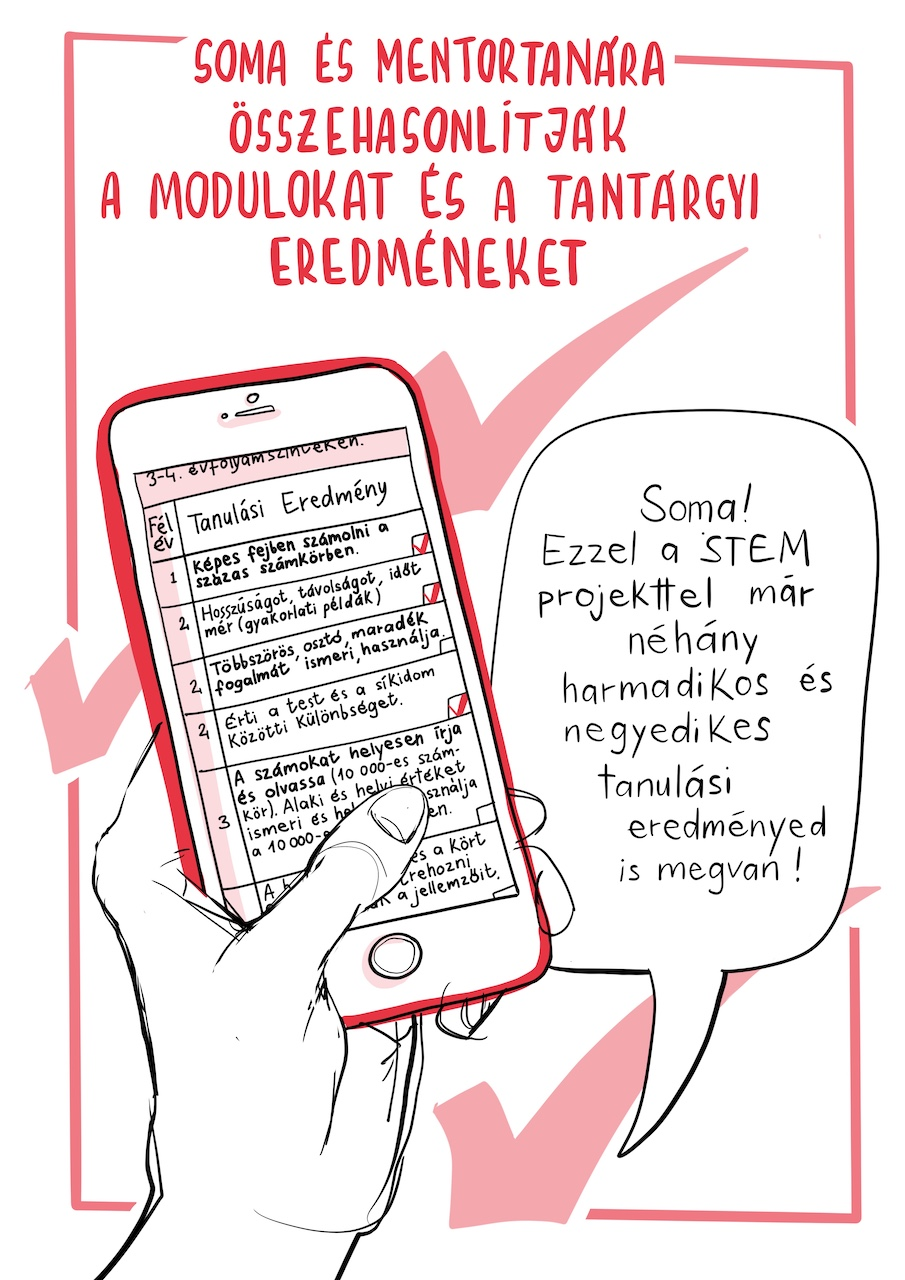
\includegraphics{pics/6a_tantargyi_soma.jpg}
\caption{Tanulási eredmények elszámolása}
\end{figure}

\hypertarget{uj-tanulasi-eredmenyek}{%
\paragraph{Új tanulási eredmények}\label{uj-tanulasi-eredmenyek}}

A gyerekek olyan tanulási eredményt is elérhetnek, ami a modulok céljai
között eredetileg nem volt megadva, mert

\begin{itemize}
\item
  lehetőségük van egyénileg is tanulni;
\item
  tanulási eredményekkel járnak a projektek, az iskolai lét, a közösségi
  élet és még számos informális és nem-formális tanulási helyzet;
\item
  egy modul során is alakulhatnak előre nem tervezett helyzetek,\break
  amik
  hozzásegíthetik a gyerekeket tanulási eredmények eléréséhez.
\end{itemize}

Az újonnan létrejövő tanulási eredmények is bekerülnek a portfólióba.

\hypertarget{tanulasi-eredmenyek-dokumentacioja}{%
\paragraph{Tanulási eredmények
dokumentációja}\label{tanulasi-eredmenyek-dokumentacioja}}

Minden modult dokumentálni\break
kell, hogy annak célja, kitűzött eredményei
nyilvánosak legyenek a Budapest School valamennyi tanára számára, és ha
szükséges, újra meg lehessen hirdetni. A tanulási eredményeket a
modulhoz kapcsolódó terv---tény összehasonlítás alapján határozzuk
meg. Az elért eredmények újra elérhetők, amennyiben a
folyamatos fejlődés biztosítva van.

\hypertarget{egyseges-modulok-egyedi-alkalmazasa}{%
\paragraph{Egységes modulok egyedi
alkalmazása}\label{egyseges-modulok-egyedi-alkalmazasa}}

Egy modul elvégzésével a gyerekek más-más tanulási eredményt is elérhetnek.

\begin{itemize}
\item
  Működhet a differenciálás, tehát nem minden gyerek ugyanazt és
  ugyanúgy csinálja a foglalkozásokon. Egy modulban tud együtt tanulni
  az a gyerek, aki még a \emph{„Hangokból, szótagokból szavakat épít''}
  eredményért dolgozik, és az, aki \emph{„Értő figyelemmel követi a
  tanító, illetve társai felolvasását.''}
\item
  A modulnak része lehet testre szabható sáv is. Például egy tudományos
  kísérletező modulban néhány gyerek a rövid távú memória és a fáradtság
  kapcsolatát kutatja, a másik csoport az esőzés és a közlekedési dugók
  kialakulása közti kapcsolatot vizsgálja. Minden gyerek elérheti a
  \emph{„Megérti a környezetében jelen lévő logikai, mennyiségi,
  függvényszerű, térbeli és statisztikai kapcsolatokat''} (Matematika 9--12.) eredményt, de a két különböző kutató csapat más-más
  területen dolgozik, így más témában merül el.
\item
  Egy-egy gyerek saját tanulási célja érdekében extra lépéseket tehet,
  és olyan eredményeket is el tud érni, amit mások nem. Például egy
  modul végén önálló prezentációt, saját kutatási tervet vagy egy kész
  működő modellt alkothat.
\end{itemize}

\hypertarget{tanulasi-eredmenyek-elerese}{%
\subsection{Tanulási eredmények
elérése}\label{tanulasi-eredmenyek-elerese}}

A tanulási eredményt sokféleképpen tekinthetjük elértnek.

\begin{itemize}
\tightlist
\item
  A modulok végeztével a tanárok igazolhatják a tanulási eredmény
  elérését.
\item
  Kihívások, tudáspróbák, tesztek, szabványos vizsgák teljesítése
  szintén megadott tanulási eredmény elérést igazolja.
\end{itemize}

Az elért tanulási eredmények bekerülnek a portfólióba. Így mindig nyomon
követhető, hogy mi és ki igazolja a tanulási eredmény elérésének tényét.

\hypertarget{ha-nincsenek-meg-a-tanulasi-eredmenyek}{%
\paragraph{Ha nincsenek meg a tanulási
eredmények}\label{ha-nincsenek-meg-a-tanulasi-eredmenyek}}

Az elért tanulási eredmények listája a portfólióban bármikor bővíthető.
Egy feladatlap kitöltése, egy tudáspróba, egy vizsga (akár online
vizsga) mind-mind tanulási eredmények elérésének bizonyítékai. Ha a
portfólió alapján nem állapítható meg az évfolyam teljesítéséhez és az
osztályzathoz szükséges tanulási eredmények megléte, akkor a gyereknek
ki kell egészítenie a portfólióját.

Ugyancsak kiegészítendő a portfólió, ha igazolt vagy igazolatlan
mulasztások miatt az iskolában végzett munka nem volt elegendő az
elégséges portfólió-elemek összegyűjtésére. Ez azt is jelenti, hogy az
iskolának nem kell a fenti folyamattól, folyamatoktól eltérnie, csak a
portfóliót kell kibővíteni.
